%\subsubsection{TOTUS data store setup}
%Figure \ref{fig:totus_setup_flow} shows the workflow to setup the data store for TOTUS.
%\begin{landscape}
%	\begin{figure}[h]
%		 \caption{TOTUS setup workflow}
%		 \label{fig:totus_setup_flow}
%		 \missingfigure{Workflow diagram for TOTUS setup and data loading}
%		  %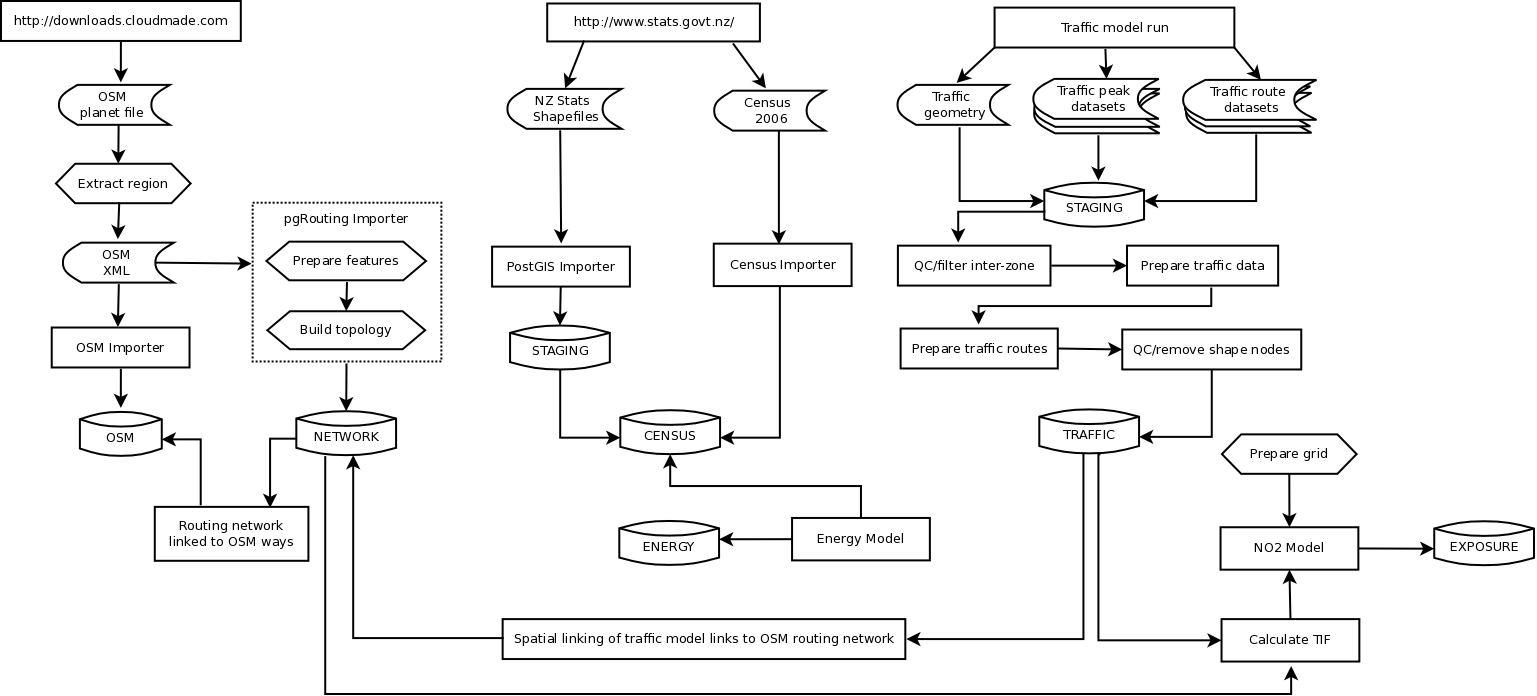
\includegraphics[width=\linewidth]{./system_preparation.png}
%		   % system_preparation.png: 1537x696 pixel, 51dpi, 76.85x34.80 cm, bb=0 0 2178 986
%	\end{figure}
%\end{landscape}

The primary data source of TOTUS is the Open Street Map (OSM) dataset. The TOTUS
loader requires an OSM \textit{planet file} for the area of interest. These data are then imported to the \textit{osm}  and \textit{network} schemas.  All routing edges (\textit{network}) are linked with their OSM counterparts to allow modifications of the OSM to used any other attributes or spatial features of interest to TOTUS.

The next step is to load the traffic model dataset defined to be compatible with traditional strategic traffic modelling packages (EMME, CUBE, etc). This dataset consists of two set of files. The first is shape files defining the traffic model zones and the modelled links both in terms of their geometry and their attributes. The second one is spreadsheets that contain all the traffic attributes for each link and for each traffic period modelled. Although not required, public transport information can be loaded in a similar fashion to traffic modelling data.

Once the traffic model data is loaded, it needs to be linked to the \textit{osm} schema. This is not a trivial exercise if the \textit{links} in the traffic model do not accurately represent the geometry of the road network. The linking process used in TOTUS is described elsewhere\cite{dummy_temp}\todo{MAKE THIS REFERENCE APPEAR!!!}. 

Finally, the census data, provided as spreadsheets, is loaded using the TOTUS census importer. The census
database schema in TOTUS holds demographic data for a set of topics
each with their own categories. Each category consist of one or more
classes, each of which may be assigned a count per mesh-block area.

\todo[inline]{Statement on the availability and accessibility of the code ... DOI for the repo?}